\documentclass[12pt,fleqn]{book}
\usepackage{amsmath} %utk masuk begin{align}
\usepackage{breqn}
\usepackage{amsxtra}%supaya \eqref
\usepackage{amsopn}%supaya dapat declare benda baru \citep
\usepackage{amsbsy}
\usepackage{amstext}
\usepackage{amsfonts}
\usepackage{amssymb}
\usepackage{amsthm}
\usepackage{shadow}% kotak shadow
\usepackage{chaptengah}
\usepackage{curves}
\usepackage{graphicx}
\usepackage{color}%masukan color
\usepackage{maple2e}
%\usepackage{flafter}
\usepackage{afterpage}
%\usepackage{tocloft}
\usepackage{XTocinc}% utk center contents, masuk chapter, topic dan page number
%  bila masuk ini jadi bold tex
%\usepackage[bottom=0.5in]{geometry}
\usepackage{lipsum}
\usepackage{imakeidx}
\makeindex
%-----------------------
\usepackage{titletoc} 
\makeatletter
\renewcommand*{\@dotsep}{999}% untuk buang dotted line besar nombor spt spt 999
\makeatother
\newtheorem{ts}{Task}
%------------------------
%--------%---
%
%\titlecontents{section}[1.5em]
 % {\bfseries}
  %{\contentslabel{2em}}
  %{\hspace*{-2.3em}}
  %{\titlerule*[1pc]{.}\contentspage} 
\usepackage{natbib}
\usepackage{enumitem}
%\makeindex
 \citestyle{mn}%\documentclass[11pt,fleqn]{report}

%\usepackage{mn}
\theoremstyle{plain}
\newtheorem{thm}{Theorem}[section]
\newtheorem{cor}[thm]{Corollary}
%\newtheorem{lem}[thm]{Lemma}
\newtheorem{prop}[thm]{Proposition}
%
%\theoremstyle{Example}
\newtheorem{exl}{Example}[section]
%
\newcommand{\sn}{\textbf{Solution}}
\theoremstyle{plain}
%\newtheorem{thm}{Theorem}[section]
%\newtheorem{cor}[thm]{Corollary}
%\newtheorem{lem}[thm]{Lemma}
%\newtheorem{prop}[thm]{Proposition}
%
\theoremstyle{Example}
%\newtheorem{exl}{Example}%section]
\theoremstyle{Question}
\newtheorem{qs}{Question}
\theoremstyle{Task}
%\newtheorem{ts}{Task}
\theoremstyle{Solution Task}
\newtheorem{sots}{Answer}
\theoremstyle{Exercise}
\newtheorem{ex}{Exercise}%section]

%
\theoremstyle{definition}
\newtheorem{defn}{Definition}[section]
%
\theoremstyle{solution}
\newtheorem{so}{Solution}
%\theoremstyle{}
%\newtheorem{qs}{}[]

\theoremstyle{remark}
\newtheorem{rem}{Remark}[section]
\newcommand{\Lim}{\mathop{\mathrm{\lim}}\limits}

%


%\theoremstyle{Problem Solving}
\newtheorem{prob}{Problem Solving}[chapter]
%
%\theoremstyle{Solution to Problem}
\newtheorem{sop}{Solution to Problem Solving}[chapter]
%
%\theoremstyle{Solution}
%\newtheorem{so}{Solution}[section]
%---------
%
%\newcommand{\Lim}{\mathop{\mathrm{\lim}}\limits}
\newcommand{\A}{\mathop{\mathrm{A}}\limits}
\newcommand{\B}{\mathop{\mathrm{B}}\limits}
\newcommand{\C}{\mathop{\mathrm{C}}\limits}
\newcommand{\D}{\mathop{\mathrm{D}}\limits}
\newcommand{\E}{\mathop{\mathrm{E}}\limits}
\newcommand{\ra}{\mathop{\longrightarrow\longrightarrow}\limits}

%\theoremstyle{Question}
%\newtheorem{qs}{Question}
%------------------
%\theoremstyle{definition}
%\newtheorem{defn}{Definition}[section]
%
%\theoremstyle{Key Term}
\newtheorem{term}{Key Term}[section]

%\theoremstyle{remark}
%\newtheorem{rem}{Remark}[section]
%
%\newtheorem{exl}{Example}[section]
%\newtheorem{so}{Solution}[section]
%\newtheorem{la}{\mathfrak{L}\{\}}[section]
\newcommand{\lap}{\mathop{\mathfrak{L}}\limits}
%--------------------
\newcommand{\mut}{\mathop{\mathfrak{U}}\limits}
\newcommand{\lapi}{\mathop{\mathfrak{L}^{-1}}\limits}
\DeclareMathOperator*{\argmin}{argmin}
\DeclareMathOperator*{\argmax}{argmax}
%---------

\oddsidemargin 0.6cm \evensidemargin 0in
%\addtolength{\hoffset}{3.0cm}
\marginparwidth 15pt \marginparsep 7pt
\topmargin 1.5cm %asal1.5
\headsep 1.0cm %asal 1.1
\addtolength{\voffset}{-2.6cm}%adjust 1.25m page no. dari tepi atas
\textheight 22.0cm \textwidth 16.0cm %asal 25.2
%\voffset=0.25cm
\headheight=13pt
\setcounter{chapter}{0}
\pagestyle{headings}
%\pagestyle{plain}
%\setcounter{page}{8}
\begin{document}
\setcounter{tocdepth}{4}    %How many levels to include in TOC
\addtocontents{toc}{\protect\sloppy}    %Keeps long chapters within page # margins
\pagenumbering{roman}
\tableofcontents
\pagenumbering{arabic}
\setcounter{chapter}{0}
\chapter{Vehicle Models}
\section{Unicycle model}

\begin{align}
\dot{x} &= u_s\cos{\theta}\\
\dot{y} &= u_s\sin{\theta}\\
\dot{\theta} &= u_\omega
\end{align}
\subsection{Reed Shepp's Car}
A Unicycle model can simulate a Reed-Shepp's car with 
\begin{itemize}
    \item $u_s \in \{-1, 0, 1\}$
    \item Transformation $u_{\omega}=\frac{\tan{\delta}}{L}$
    \item restricting $\delta$ to $[-\delta_{max}, \delta_{max}]$ where $\delta$ represent the steering angle and $\frac{L}{\tan\delta}$ represents the turning radius. $L$ is the wheel-base.
\end{itemize} 
\subsection{Dubin's Car}
Dubin's car is a simplification of Reed-Shepp's car  with $u_s \in \{0, 1\}$ 

\shabox{A unicycle model can simulate a Reed-Shepp's car, Dubin's car and the Single track rear wheel model below when steering is the control input without considering the steering rate. It can also simulate tricycle and differential drive robot. The details are not discussed here explicitly}

\section{Single Track Rear Wheel Model}
For a front-wheel driven vehicle with no slip
\begin{align}
\dot{x} &= u_s\cos{\theta} \\
\dot{y} & = u_s\sin{\theta} \\
\dot{\theta} & = u_s \frac{\tan{\delta_r}}{L} \\
\dot{\delta_r} &= u_\delta
\end{align}
where $L$ is the wheel base and the state represents the rear-wheel, $\delta_r$ represents the steering angle at the rear wheels and $u_s$ is the speed of the rear-wheel

The Single track rear wheel model can be further expanded out to include acceleration  as
\begin{align}
\dot{x} &= u_s\cos{\theta} \\
\dot{y} & = u_s\sin{\theta} \\
\dot{\theta} & = u_s \tan{\delta_r}/L \\
\dot{u_s} &= u_a \text{(or other first order approximations/reduced order models)} \\
\dot{\delta_r} &= u_\delta
\end{align}
the control input is $u=[u_a  u_\delta]^{'}$
If curvature is the input to the system, the model can be rewritten as
\begin{align}
\dot{x} &= u_s\cos{\theta} \\
\dot{y} & = u_s\sin{\theta} \\
\dot{\theta} & = u_s \kappa \\
\dot{u_s} &= u_a \text{(or other first order approximations/reduced order models)}
\end{align}
where $\kappa$ indicates the curvature value
\section{Single Track Front Wheel Model}
For a front-wheel driven vehicle with no side slip
\begin{align}
\dot{x} &= u_s\cos({\theta + \delta}) \\
\dot{y} & = u_s\sin({\theta + \delta}) \\
\dot{\theta} & = u_s \frac{\sin{\delta}}{L} \\
\dot{\delta_f} &= u_\delta
\end{align}
where $\delta_f$ represents the steering angle at the front wheels wheels.
This model can be augmented with acceleration commands instead of speed similar to the equations presented in the rear wheel models.

Furthermore, the models can be rewritten using curvature instead of steering angles or steering rate. Additionally, there are limits on speed, acceleration, steering, steering rate and curvature.
\section{Model with Slip}
Assuming the vehicle can be steered with both front and rear wheels, the model equations with slip $\beta$ are
\begin{align}
\dot{x} &= u_s\cos(\theta+\beta) \\
\dot{y} &= u_s\sin(\theta+\beta) \\
\dot{\theta} &= u_s\frac{\cos{\beta}}{l_f+l_r}(\tan\delta_f - \tan\delta_r) \\
\dot{u_s} &= u_a \\
\beta & = \arctan(\frac{l_f\tan\delta_r+l_r\tan\delta_f}{l_f+l_r})
\end{align}
where $\beta$ denotes vehicle slip angle, $l_f$ is the distance of the front wheels to the center of mass, $l_r$ is the distance of the rear wheels to the center of mass, $\delta_f$ is the front wheel steer and $\delta_r$ is the rear wheel steer
\begin{figure}[!ht]
\centering
 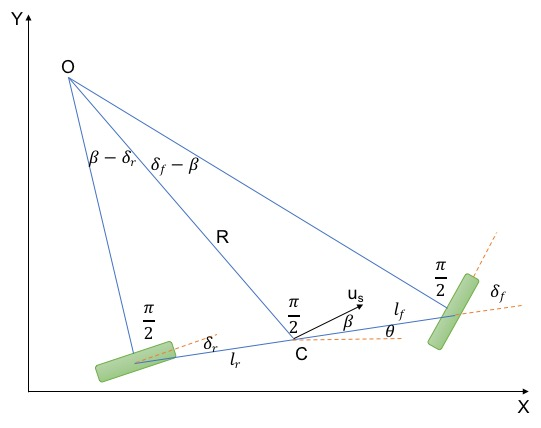
\includegraphics[width=0.8\textwidth]{slip_kinematic_model.jpg}   
\caption{Kinematic vehicle model with Slip and front and rear wheel steer. O is the instantaneous center of rotation} \label{fig:slip_kin_model}
\end{figure}
\subsection{Derivation}
From left triangle, applying the sine rule
\begin{align}
    \frac{\sin(\frac{\pi}{2}+\delta_r)}{R} &= \frac{sin(\beta-\delta_r)}{l_r} \\
    \implies \frac{l_r}{R} &= \sin\beta - \tan\delta_r\cos\beta \label{eq:rear_slip_beta}
\end{align}
From the triangle on the right, applying the sine rule
\begin{align}
    \frac{\sin(\frac{\pi}{2}-\delta_f)}{R} &= \frac{sin(\delta_f - \beta)}{l_f} \\
    \implies \frac{l_f}{R} &= \tan\delta_f\cos\beta - \sin\beta  \label{eq:front_slip_beta}
\end{align}
Divide equations (\ref{eq:rear_slip_beta}) and (\ref{eq:front_slip_beta}), we have
\begin{align}
    \frac{l_r}{l_f}&=\frac{\sin\beta - \tan\delta_r\cos\beta}{\tan\delta_f\cos\beta - \sin\beta} \\
    \implies \frac{l_r}{l_f}&=\frac{\tan\beta-\tan\delta_r}{\tan\delta_f - \tan\beta} \\
    \implies \tan\beta &= \frac{l_r\tan\delta_f + l_f\tan\delta_r}{l_f+l_r}
\end{align}
Now we know that $\dot{\theta}=\frac{u_s}{R}$. To derive $R$, we use (\ref{eq:rear_slip_beta}). Substituting $\tan\beta$ derived above into \ref{eq:rear_slip_beta}, we have
\begin{align}
    \frac{l_r}{R} &= \cos\beta(\tan\beta - \tan\delta_r) \\
    \implies \frac{l_r}{R} &= \cos\beta(\frac{l_r\tan\delta_f + l_f\tan\delta_r}{l_f+l_r} - \tan\delta_r) \\
    \implies \frac{l_r}{R} &= \frac{\cos\beta}{l_f+l_r}(l_r\tan\delta_f - l_r\tan\delta_r) \\
    \implies \frac{1}{R} &= \cos\beta\frac{\tan\delta_f - \tan\delta_r}{l_f+l_r} \\
    \implies \dot{\theta}&=\frac{u_s}{R}= u_s\cos\beta\frac{\tan\delta_f - \tan\delta_r}{l_f+l_r}
\end{align}
As far the equations for $x$ and $y$ go, it is straightforward to see that
\begin{align}
    \dot{x}&=u_s\cos(\theta+\beta) \\
    \dot{y}&=u_s\sin(\theta+\beta) \\
\end{align}

\section{Dynamic Lateral and Longitudinal Model} 
\subsection{Lateral Dynamics}
The lateral dynamics is given by
\begin{align}\label{eq:lat_dynamics}
    ma_y &=m\Ddot{y} + u_{sx}\dot{\theta} = F_{yf} + F_{yr} + F_{bank} \\
    I_z\Ddot{\theta} &= l_fF_{yf}-l_rF_{yr}
\end{align}
where $F_{yf}$ and $F_{yr}$ denote the lateral tire forces at the front and rear wheels, $m$ is the mass of the vehicle, $u_sx$ is the longitudinal speed of the vehicle at CG. 

\shabox{Slip is the difference in angle between velocity vector at the wheel and the steering angle}

For small slip angles (i.e. lower speeds <~35-40 mph typically for nominal friction conditions i.e no sleet, water, ice etc), they are approximated by (for front wheel drive) a linearly as.
\begin{align}
    F_{yf} &= 2C_{\alpha f}(\delta-\theta_{vf}) \\
    F_{yr} &= 2C_{\alpha r}(-\theta_{vr})
\end{align}
where $C_{\alpha f}$ and $C_{\alpha r}$ represent the cornering stiffness of each of the front and rear wheels respectively.
$F_{bank} = mg\sin\phi$, where $\phi$ is the bank angle, $g$ is the acceleration due to gravity
The velocity vector at the wheels are given by
\begin{align}
    \tan{\theta_{vf}} &= \frac{u_sy+l_f\dot{\theta}}{u_sx} \\
    \tan{\theta_{vr}} &= \frac{u_sy-l_r\dot{\theta}}{u_sx}
\end{align}
Using small angle approximations, the above equations can be further reduced to 
\begin{align}
    \theta_{vf} &= \frac{\dot{y}+l_f\dot{\theta}}{u_sx} \\
    \theta_{vr} &= \frac{\dot{y}-l_r\dot{\theta}}{u_sx}
\end{align}
\subsection{Longitudinal Dynamics}
\begin{figure}
    \centering
    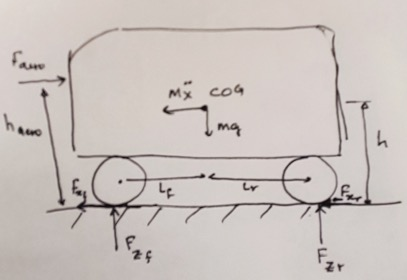
\includegraphics{veh_long_dyn.jpg}
    \caption{Longitudinal forces on the vehicle}
    \label{fig:veh_long_dyn}
\end{figure}
Ignoring the pitch of the vehicle i.e. assuming flat surface, the longitudinal dynamics is given by
\begin{align}
    m\Ddot{x}&=F_{xf} + F_{xr} - F_{aero} - R_{xf} - R_{xr}
\end{align}
where $F_{xf}$ and $F_{xr}$ denote the longitudinal forces at the front and rear wheels respectively, $F_{aero}$ denotes aerodynamics drag force, $R_{xf}$ and $R_{xr}$ denote rolling resistance at the front and rear wheels
Aerodynamic drag force is given by
\begin{align}
    F_{aero} &= \frac{1}{2}\rho C_dA_F(V_x+V_{wind})^2
\end{align}
where $\rho$ is the density of air, $C_d$ is the aerodynamic drag coefficient, $V_x$ is the longitudinal speed of the vehicle, $V_wind$ is the wind velocity and $A_F$ is the frontal area of the vehicle.
The longitudinal tire forces are a function of slip, normal load on the tire and the friction coefficient.
The longitudinal slip ratio is defined as
\begin{align}
    \sigma_{long} &= \frac{r_{eff}\omega_{wheel}-V_x}{V_x} \textsc{braking} \\
    \sigma_{long} &= \frac{r_{eff}\omega_{wheel}-V_x}{r_{eff}\omega_{wheel}} \textsc{acceleration} 
\end{align}
where $\omega_{wheel}$ is the rotational speed of the wheel and $r_{eff}$ is the effective tire radius.
When the slip is small, the longitudinal forces are given by
\begin{align*}
    F_{xf} &= C_{\sigma f}\sigma_{xf} \\
    F_{xr} &= C_{\sigma r}\sigma_{xr}
\end{align*}
where $C_{\sigma f}$ and $C_{\sigma r}$ represent longitudinal stiffness at front and rear wheels.

The rolling resistance $R_{xf}$ and $R_{xr}$ are approximated using the coefficient of friction and the normal loading force at the front wheel $F_{zf}$ and rear wheel $F_{zr}$ as
$$R_{xf} + R_{xr} = f (F_{zf} + F_{zr})$$.
When the vehicle is travelling along a surface with no gradient, $F_{zf}$ and $F_{zr}$ are in turn calculated by taking moments about the contact points of the front and rear wheels as 
(see Figure~\ref{fig:veh_long_dyn}) 
\begin{align}
    F_{zf}(l_f+l_r) + F_{aero}h_{aero} -m\Ddot{x}h - mgl_r &= 0 \\
    F_{zr}(l_f+l_r) - F_{aero}h_{aero} +m\Ddot{x}h - mgl_f &= 0 
\end{align}
The above equations can be straightforwardly extended to the case when the vehicle is pitching while maintaining contact with the ground i.e when the vehicle is moving on an inclined surface. (the terms that correspond $mg$ will have additional component along and perpendicular to the surface)
\subsection{Error models}
\subsubsection{With respect to the road}
Let's say the objective is to follow the center line of the road. At any given point let $\theta_{des}$ be the headong of the centerline. The lateral acceleration desisred at this point would be $V_x\theta_{des}$. The lateral acceleration of the vehicle in the inertail coordinates is $a_y = \Ddot{y} + V_x\theta$ where $V_x$ is the longitudinal speed of the vehicle in the body frame and $\theta$ is the heading of the vehicle. The error equations under the assumption of constant longitudinal speed can be written as
\begin{align}
    \dot{e_1} &= \Ddot{y} + V_x(\dot{\theta} - \dot{\theta_{des}}) \\
    \dot{e_2} & = \dot{\theta} - \dot{\theta_{des}}
\end{align}
where $e_1 = \dot{y} + V_x(\theta - \theta_{des})$ and $e_2 = \theta - \theta_{des}$
The error dynamics can now be obtained using~(\ref{eq:lat_dynamics}). The model now can be used for developing steering control law the objective of which would be to stabilize the above system.
\section{Linearization}
Let's say a dynamic system is defined by
\begin{align}
    \dot{x} &= f(x, u)
\end{align}
where $x$ is the state and $u$ is the control input
The linearized system is given by
\begin{align}
    \dot{\delta x} = \frac{\partial f}{\partial x} \delta x + \frac{\partial f}{\partial u} \delta u + H.O.T
\end{align}
H.O.T (Higher order terms) are generally neglected under the assumption that $\delta x$ and $\delta u$ are small. Linearization is generally used for stability analysis and for designing controllers for reference and trajectory tracking (example LQR, MPC etc) 

First define $\delta x = x - x^{*}$ and $\delta u = u - u^{*}$ where $x^*$ and $u^*$ represent the state and control inputs at equilibrium  or define the operating points i.e. trim conditions.
The derivation proceeds as follows
\begin{align}
    \dot{\delta x} &= \dot{x} - \dot{x^*} \\
    \implies \dot{\delta x} &= f(x, u) - f(x^*, u^*) \\
    \implies \dot{\delta x} &= f(x^* + \delta x, u^* + \delta u)- f(x^*, u^*)
\end{align}
Taylor series expansion can now be used to derive the equations above. 

H.0.T some times are used to a second degree in methods like DDP (Differential Dynamic Programming).We will discuss more about this in another chapter. 

\subsubsection{Example}
Let's take the example of the simplified single track rear wheel model. The equations for the simple car model are given by
\begin{align*}
    \dot{x} &= u_1\cos{\theta} \\
    \dot{y} &= u_1\sin{\theta} \\
    \dot{\theta} &= u_1\frac{\tan u_2}{L}
\end{align*}
where $u_1$ is the speed control input and $u_2$ is the steering control input with $L$ as the wheel base.

Using the derivation, let's linearize the system about the state $[{}0,{}0, {}pi/4{}]$ and control $[{}1, {}0{}]$
\begin{align}
    \dot{\delta x} &= 0 \times \delta x + 0 \times \delta y - (u_1=1)\times\sin(\theta = \frac{pi}{4}) \times \delta \theta + \delta u_1 \\
    \dot{\delta y} &= 0 \times \delta x + 0 \times \delta y + (u_1=1)\times\cos(\theta = \frac{pi}{4}) \times \delta \theta + \delta u_1 \\
    \dot{\delta \theta} &=  0 \times \delta x + 0 \times \delta y + 0\times\delta \theta + \frac{\tan (u_2=0)}{L} \times \delta u_1+ (u_1=1)\times\frac{\sec^2 (u_2=\frac{pi}{4})}{L}\times\delta u_2 
\end{align}
In matrix form it can be represented as
\begin{align}
    \begin{bmatrix}
          \dot{\delta x}\\
          \dot{\delta y} \\
         \dot {\delta \theta}
    \end{bmatrix} & =  \begin{bmatrix}
    0 & 0 & -\frac{1}{\sqrt{2}} \\
    0 & 0 & \frac{1}{\sqrt{2}} \\
    0 & 0 & 0
    \end{bmatrix}
    \begin{bmatrix}
          \delta x\\
          \delta y \\
         \delta \theta
    \end{bmatrix} + \begin{bmatrix}1 & 0 \\ 1 & 0 \\ 0 & \frac{2}{L}\end{bmatrix}\begin{bmatrix}\delta u_1 \\ \delta u_2\end{bmatrix}
\end{align}

\shabox{The controllability rank condition is not met by the linearized system. However the original nonlinear model i.e. the simple car model is Small Time Locally Controllable (STLC) - we will talk about this later}
%--------------
\chapter{Control}
\section{PID}
\section{LQR}
Linear Quadratic Regulator is an optimal controller for linear systems and a quadratic cost function. It drives the states to zeros while keeping the control input small. It can be extended to
\begin{enumerate}[topsep=0pt,itemsep=2pt,parsep=0pt,partopsep=0pt]
    \item Regularization of non-linear system to a non-zero fixed point
    \item Penalize rate of change of control inputs i.e for example jerk
    \item Trajectory tracking for non-linear systems
    \item Linear Time Varying (LTV) systems
    \item Stochastic Systems
    \item Affine systems
\end{enumerate}
\subsection{Problem formulation}
The finitie horizon LQR problem is to find control inputs that minimizes 
\begin{align}
    J=\sum_{k=0}^N(x_k^TQx_k + u_k^TRu_k) \label{eq:chap2_lqr_cost}
\end{align}

with $Q\succ0$ and $R\succ0$, $Q$ and $R$ are positive semi-definite matrices, subject to 
$$x_{k+1}=Ax_{k}+Bu_{k}$$
When $N$ is $\inf$, the problem is infinite horizon problem.
Since $Q$ and $R$ are positive semi-definite, any $x$ or $u$ that are not zeros will yield a positive cost by definition.
\subsection{Examples}
\subsubsection{Leader following}
For this problem, let's consider kinematic models in 1D. (The 2D motion can be reduced to under the assumption that the leader and the ego do not have any lateral movement and move on a straight road and appropriately attaching a coordinate system). Assuming our prediction module is perfect, we will model the leader as
\begin{align}
    s_{k+1}^{leader} &= s_{k}^{leader} + v_{k}^{leader} \delta t \\
    v_{k+1}^{leader} &= v_{k}^{leader}
\end{align}
$v_{k}$ is the longitudinal speed of all vehicles and is known at all time steps (from an on-board perception module).
The ego or the self vehicle that is controlled is modeled as
\begin{align}
    s_{k+1}^{ego} &= s_{k}^{ego} + v_{k}^{ego}~\delta t + 0.5~a_{k}^{ego}~\delta t^2 \\
    v_{k+1}^{ego} &= v_{k}^{ego} + a_{k}^{ego}~\delta t \\
    a_{k+1}^{ego} &= u_{k}^{ego}
\end{align}
where $u_{k}$ is the control input to our system.
The goal is to follow the leader while maintaining a distance greater than or equal to $L_{sep}$. Let's redefine the state of our system as
\begin{align}
    s_{k+1} &= s_{k+1}^{leader} - s_{k+1}^{ego} - L_{sep} \\
    v_{k+1} &= v_{k+1}^{leader} - v_{k+1}^{ego} \\
    a_{k+1} &=  - u_{k}^{ego} 
\end{align}
Rewriting the matrix form with $x_{k}=\begin{bmatrix}s_{k} \\ v_{k} \\ a_{k}\end{bmatrix}$, the system is defined by
\begin{align}
    x_{k+1} &= Ax_{k} + Bu_{k}
\end{align}
with $$A=\begin{bmatrix}1 & \delta t & 0.5\delta t^2 \\ 0 & 1 & \delta t \\ 0 & 0 & 0 \end{bmatrix}$$ and $$B=\begin{bmatrix} 0 \\ 0\\ -1 \end{bmatrix}$$. The goal is to drive the system states to zeros while minimizing the control effort. In this formulation, the control effort gets penalized twice as it is part of the state as well. So $Q$ and $R$ should be chosen carefully.

\shabox{Notice that in the formulation, there is nothing preventing ego vehicle from crossing the leader and then maintaining $L_{sep}$ apart from the control cost. There is also nothing preventing the system from commanding high acceleration or deceleration between consecutive steps $\implies$ uncomfortable ride. (which could happen based on the initial conditions)}


One way to address the second problem is to increase entries in $R$ i.e. penalize control effort a lot but this will also imply slow convergence and still nothing prevents it from giving large $\delta u$. To address this issue one can penalize $\delta u$ in the cost function. The problem can be reformulated with $\delta u$ as the control input i.e rate of change of acceleration as control input. The equations are now
\begin{align}
    s_{k+1} &= s_{k+1}^{leader} - s_{k+1}^{ego} - L_{sep} \\
    v_{k+1} &= v_{k+1}^{leader} - v_{k+1}^{ego} \\
    a_{k+1} &=  a_{k} + u_{k-1}^{ego}- u_{k}^{ego} \\
    \implies a_{k+1} &= a_{k} - \Delta u_{k}
\end{align}
where $\Delta u_{k} = u_{k}^{ego}- u_{k-1}^{ego}$
In matrix form the $A$ and $B$ matrices are transformed to

The typical way to go about penalizing change in control inputs for this problem is to initially start with $x$ as two states (position and speed), then augmenting the state vector with control input as the third state (position, speed and acceleration/control input) and a change in the control input (change in acceleration) as the control input.
\iffalse
\begin{align}
    x'_{k+1} &= A'x'_{k} + B'u'_{k}
\end{align}
with $x'_{k}=\begin{bmatrix}s_{k} \\ v_{k} \\ a_{k} \\u_{k}\end{bmatrix}$
, $A'=\begin{bmatrix}1 & \delta t & 0.5\delta t^2  & 0\\ 0 & 1 & \delta t & 0\\ 0 & 0 & 0 & -1 \\ 0 & 0 & 0 & 1 \end{bmatrix}$ and $B'=\begin{bmatrix} 0 \\0 \\ -1 \\ 1 \end{bmatrix}$ and $u'_{k}=u_{k} - u_{k-1}=\Delta u_{k}$
\fi
\subsubsection{Trajectory tracking}
\paragraph{Problem} The trajectory tracking problem is to compute a sequence of control input $u_1, u_2, ..., u_{H-1}$ so that a state sequence $x_0^*, x_1^*, ..., x_H^*$ is attainable such that $x_{t+1}=f(x_t, u_t)$ while minimizing the cost function $\sum_{i=0}^{H-1}(x_i - x_i^*)^T Q (x_i - x_i^*) + (u_i - u_i^*)^T R (u_i - u_i^*)$ where $u_i^*, i=0 to H-1$ is a control input that ensures feasibility i.e. $x_{t+1}^*=f(x_t^*, u_t^*) {} \forall t \in \{0, 1, ..., H-1\}$
\paragraph{Example}
The trajectory tracking problem for non-linear systems can be transformed to LQR for Linear Time Varying case via linearization. If the input trajectory is not feasible, the computed solution will not visit the desired states.
Let's consider the example of cruise control. The objective is to regulate the longitudinal speed of the vehicle using LQR. In this case, it is sufficient to consider longitudinal dynamics alone. Let the reference speed to be tracked be given by
\begin{align}
    v(t) &= 10|\sin(0.2\pi t)| \label{chap_2:eq:vel_traj}
\end{align}
Assuming that there is no wind and no gradient, the simplified longitudinal dynamics can be written as
\begin{align}
    m\dot{v} &= u - F_{friction} - F_{drag}  \label{chap_2:eq:long_traj_tracking}\\ 
\end{align}
For the sake of simplicity, let's consider the RMS of speed and acceleration and to derive the nominal control input. RMS is the value that the system will see when the input is applied.
The following parameters will be used 
\begin{itemize}
\item[] $m = 1000$
\item[] $\rho = 1$
\item[] $C_d =0.6$
\item[] $A = 3$
\item[] $C_r=0.3$
\item[] $V_{rms} = 10/\sqrt{2} = 7.07$
\item[] $F_{drag} = 0.5 * \rho * A * C_d * V_{rms}^2$ $\implies$ $F_{drag}=44.98 N$, 
\item[] $F_{friction}=C_r*V_{rms}$ $\implies$ $F_{friction}=2.12 N$. 
\item[] RMS of acceleration $\dot{v}$ is $0.45$.
\end{itemize}
The nominal control input $u = 1000 * 0.45 + 44.98 + 2.12$ i.e. $u^{*}=497.1 N$.

Next let's linearize the system around the nominal control input and the state at time $t$.
Using the method discussed in Section~\ref{chap_1:sec:linearization}, the linearized model is
\begin{align}
    m\dot{\delta v} &= \delta u - C_r  \delta v - \rho C_d  A  v  \delta v \label{chap_2:eq:linearized_long_traj_tracking} 
\end{align}
where $v$ represents the operating point at which linearization is performed
Let's now verify the accuracy of linearization when $v=10$ $\implies$ $\dot{v}=-0.45$ and $\delta v = 2.93$
\begin{enumerate}
    \item Using (~\ref{chap_2:eq:long_traj_tracking}), we get $u=93$ $N$ 
    \item Using (~\ref{chap_2:eq:linearized_long_traj_tracking}), we have $\dot{\delta v} = -0.45$, $\delta v = 10-7.07=2.93$ $\implies$ $\delta u = -450 + 0.879 + 52.74 = -396.38 $. From this $u = u^{*} + \delta u = 497.1 - 396.38 = 100.72$ $N$
    \item The estimates are close but not close enough. This is because $\delta v = 2.93$ is a large number. The contributions of the Higher Order Terms (H.O.T) which were neglected in the linearization will contribute to errors. So, when linearizing make sure that the $\delta$'s are small. Had we chosen the operating point to be $8 m/s$, the estimates would be much closer. The resolution of discretization used to solve the problem affects the accuracy of linearization.
\end{enumerate}

Now let's design the cost function for this example. To make life easier and avoid integrals, lets discretized the linearized system. The equations for the discretized system are given by
\begin{align}
    m\delta v_{k+1} = m\delta v_{k} - C_r \delta v^{*}_{k} \delta t - \rho C_d A v \delta v_{k} + u \delta t \\
    \implies
    \delta v_{k+1} = \left(1 - \frac{C_r \delta t}{m} - \frac{\rho C_d A v_{k}^{*} \delta t}{m}\right)\delta v_{k} + \delta u \delta t
\end{align}
where $\delta t$ is the sampling time and $v_{k}^{*}$ is the target/desired speed at time step $k$
The cost function for the above system is of the form
\begin{align*}
    \sum_{k=1}^{N}q\left(v_{k} - v^{*}_{k}\right)^2 + \sum_{k=1}^{N}r\left(u_{k} - u^{*}_{k}\right)^2
\end{align*}
where $N$ is the horizon. For example, if the time horizon we are looking at $T$=$5$ seconds, and $dt=0.1$, then $N=50$, $q$ is the penalty on state deviation and is a scalar (since the system is 1D) and $r$, is the penalty on control input deviation and is a scalar (1D).
$v_{k}^{*}$ is determined by~(\ref{chap_2:eq:vel_traj}) and $u_{k}^{*} = 497.1$ $\forall$ $k$ $\in$ $\{1, 2, 3, ... N\}$.


In this specific example we chose $q=10$ and $r=1$. We chose a low $r$ allow deviation in control as it is not a feasible control input for the states we want to visit. We chose a high $q$ (compared to $r$) as we would like to get sufficiently close to the desired state sequences.

\shabox{If the input trajectory is feasible, why do we need LQR?. For example, in the above case, open loop control inputs can be computed by inverting the dynamics as a function of the desired states. If we did this, why doe we need LQR - use the computed control input directly.}


Generally, approximate trajectory (state and control) is computed using a reduced order model of the system. Such an approach gets the state and control sequences close to a feasible/optimal trajectory. Then LQR (or another approach) can be used with higher order model dynamics to improve the controls. One should also be careful in aligning the cost functions across various stages of development. The general approach is to segment the problem into path, trajectory and control modules where the solution from one module feeds into the other improving it successively via additional constraints and model order with appropriate cost functions. There are other reasons too and this is one of them. 

In the example above, we could augment the system with additional equations for representing the lower level control. For example the computed control input might not be translated or transferred to the actuators instantaneously. One could use a first order model to represent the system. But using the model could complicate trajectory generation module. So, partitioning it will make life easier and could also ease compute time issues.

\subsection{Derivation}
\subsubsection{Dynamic Programming}
We will use bottom up DP approach for coming up with the solution.
We will use the following identity 
\begin{align}
    \frac{d(x^TAx)}{dx} &= x^T(A^T+A)
\end{align}
If $A$ is symmetric
\begin{align}
    \frac{d(x^TAx)}{dx} &= x^T(A^T+A)=2x^TA=2A^Tx=2Ax
\end{align}
Let's look at the equation~\ref{eq:chap2_lqr_cost}. We can write the optimization problem as
\begin{align}
    J^*(x) &= \argmin_{u_k, for k \in \{1, 2, ..., N-1\}}\sum_{k=0}^{N-1}\left[x_k^TQx_k + u_k^TRu_k \right] + x^T_NP_Nx_N
\end{align}
assuming the control input $u_N=0$
we have
\begin{align}
    J(x_{N}) &= x_N^TP_NX_N \\
    \implies J(x_N) &= (Ax_{N-1}+Bu_{N-1})^TP_N(Ax_{N-1}+Bu_{N-1})\\
    J^*(x_{N-1}) &= \argmin_{u_{N-1}}\left[x_{N-1}^TQx_{N-1} + u_{N-1}^TRu_{N-1} + J^*(x_N)\right] \\
\end{align}
\begin{dmath*}
    \implies J^*(x_{N-1}) = \argmin_{u_{N-1}}\left[x_{N-1}^TQx_{N-1} + u_{N-1}^TRu_{N-1} +  (Ax_{N-1}+Bu_{N-1})^TP_N(Ax_{N-1}+Bu_{N-1})\right]
\end{dmath*}
As $u_{N-1}$ does not depend on $x_{N-1}$ and $J(x_{N-1})$ denotes the cost to go from $x_{N-1}$ to $x_{N}$ and $*$ denotes the optimal cost or input corresponding to the optimal cost.
For minimizing $J(x_{N-1})$, we set $\frac{\partial (x_{N-1})}{\partial u_{N-1}} = 0$ which results in
\begin{align}
    & Ru^*_{N-1} + (Ax_{N-1}+Bu^*_{N-1})^TP_NB = 0 \\
    \implies & Ru^*_{N-1} + B^TP_N(Ax_{N-1}+Bu^*_{N-1}) = 0 \\
    \implies & u^*_{N-1} = -(R+B^TP_NB)^{-1}B^TP_NAx_{N-1}
\end{align}
Now $J(x_{N-1})$ can be reloaded using the above equation as
\begin{dmath*}
    J^*(x_{N-1}) = \left[x_{N-1}^TQx_{N-1} + (K_{N-1}x_{N-1})^TR(K_{N-1}x_{N-1}) + (Ax_{N-1}-BK_{N-1}x_{N-1})^TP_N(Ax_{N-1}-BK_{N-1}x_{N-1})\right]
\end{dmath*}
with $$K_{N-1} = -(R+B^TP_NB)^{-1}B^TP_NA$$
$J^*(x_{N-1})$ can now be rewritten as 
\begin{align}
    J^*(x_{N-1}) &= x_{N-1}^TP_{N-1}x_{N-1}
\end{align}
with
$$P_{N-1}= Q+K^T_{N-1}RK_{N-1}+(A-BK_{N-1})^TP_{N}(A-BK_{N-1})$$
The above expression now can be used to comute $u^*_{N-2}$ by looking at $J(x_{N-2})$ similar to the derivation above.
This concludes the derivation using DP approach
\subsubsection{Hamiltonian}
\subsection{Relation to $H_2$ controller}
\section{MPC}
\subsection{Stability}
\section{Other}
\subsection{Feedback Linearization}
\subsection{Lyapunov Controller}
\subsection{Notes on Stability}
\chapter{Path Planning}
\chapter{Trajectory Planning}
\chapter{Behavior Planning}
\chapter{Architectures}
\chapter{General Notes}

\section{Kinematics and Dynamics}
\section{Probability}
\section{Geometry}
\section{Optimization}
\section{Control}
\section{Programming \& Algorithms}
\bibliographystyle{mn}
\bibliography{cuba}
\printindex
\end{document}